\documentclass[12pt,letterpaper]{article}

\newcommand{\projectname}{ExamGrid}
\newcommand{\projecttitle}{ExamGrid: Automated Exam Seating and Invigilation Allocation System}
\newcommand{\instructorname}{Ms. Ankitha A Nayak}
\newcommand{\instructordesignation}{Assistant Professor Grade - II}
\newcommand{\sectionname}{D}
\newcommand{\submissiondate}{20/11/2026}

\usepackage[T1]{fontenc}
\usepackage[utf8]{inputenc}
\usepackage{mathptmx}
\usepackage[scaled=0.92]{helvet}
\usepackage[letterpaper,top=2.3cm,bottom=2.3cm,left=2.5cm,right=2.5cm,headheight=16pt,headsep=14pt,footskip=30pt]{geometry}
\usepackage{setspace}
\usepackage{graphicx}
\usepackage{xcolor}
\usepackage{array,tabularx,longtable}
\usepackage{float}
\usepackage[font=small,labelsep=colon]{caption}
\usepackage{enumitem}
\usepackage{fancyhdr}
\usepackage{titlesec}
\usepackage{amsmath,amssymb}
\usepackage{listings}
\usepackage{tikz}
\usepackage[hidelinks]{hyperref}
\usetikzlibrary{shapes.geometric,shapes.misc,shapes.multipart,arrows.meta,positioning,fit,calc}

\definecolor{egnavy}{RGB}{13,59,102}
\definecolor{eggold}{RGB}{244,162,89}
\definecolor{eglight}{RGB}{232,239,247}
\definecolor{eggrey}{RGB}{90,100,117}
\definecolor{codebg}{RGB}{248,249,251}
\definecolor{codekw}{RGB}{0,51,153}
\definecolor{codestr}{RGB}{163,21,21}

\onehalfspacing
\setlength{\parindent}{0pt}
\setlength{\parskip}{8pt}
\emergencystretch=3em
\sloppy
\let\origtexttt\texttt
\renewcommand{\texttt}[1]{#1}
\setlist[itemize]{itemsep=3pt,topsep=4pt,leftmargin=1.4cm,label=\textbullet}
\setlist[enumerate]{itemsep=3pt,topsep=4pt,leftmargin=1.4cm}

\renewcommand{\thesection}{\arabic{section}}
\titleformat{\section}{\centering\sffamily\bfseries\large\MakeUppercase}{}{0pt}{}
\titlespacing*{\section}{0pt}{0pt}{14pt}
\titleformat{\subsection}{\sffamily\bfseries\normalsize}{\thesubsection}{0.5em}{}
\titlespacing*{\subsection}{0pt}{10pt}{4pt}
\newcommand{\chapter}[1]{\clearpage\refstepcounter{section}\section*{#1}\label{ch:\thesection}}
\newcommand{\chaplabel}[1]{\label{#1}}
\makeatletter
\renewcommand{\thesubsection}{\arabic{section}.\arabic{subsection}}
\@addtoreset{subsection}{section}
\@addtoreset{figure}{section}
\@addtoreset{table}{section}
\makeatother
\renewcommand{\thefigure}{\arabic{section}.\arabic{figure}}
\renewcommand{\thetable}{\arabic{section}.\arabic{table}}

\fancypagestyle{body}{
  \fancyhf{}
  \fancyhead[L]{\sffamily\bfseries\small\projectname}
  \fancyhead[R]{\sffamily\bfseries\small 2026-27}
  \fancyfoot[L]{\sffamily\bfseries\small Dept of CSE, NMAMIT, Nitte}
  \fancyfoot[R]{\sffamily\bfseries\small Page \thepage}
  \renewcommand{\headrulewidth}{1.2pt}
  \renewcommand{\footrulewidth}{1.2pt}
}
\fancypagestyle{front}{
  \fancyhf{}
  \fancyfoot[C]{\small\thepage}
  \renewcommand{\headrulewidth}{0pt}
  \renewcommand{\footrulewidth}{0pt}
}

\lstdefinestyle{java}{
  language=Java, basicstyle=\ttfamily\scriptsize, keywordstyle=\color{codekw}\bfseries,
  stringstyle=\color{codestr}, backgroundcolor=\color{codebg}, frame=single,
  rulecolor=\color{black!25}, numbers=left, numberstyle=\tiny\color{gray},
  breaklines=true, showstringspaces=false, tabsize=4, xleftmargin=1.5em, framexleftmargin=1.5em,
  morekeywords={record,var}, aboveskip=6pt, belowskip=6pt, linespread=1.0
}
\lstdefinestyle{plain}{
  basicstyle=\ttfamily\scriptsize, backgroundcolor=\color{codebg}, frame=single,
  rulecolor=\color{black!25}, breaklines=true, showstringspaces=false, columns=fullflexible,
  aboveskip=6pt, belowskip=6pt
}

\newcolumntype{L}[1]{>{\raggedright\arraybackslash}p{#1}}
\newcommand{\hd}[1]{\textbf{#1}}
\newenvironment{gridtable}[1]{\par\centering\sffamily\footnotesize\renewcommand{\arraystretch}{1.25}\tabularx{\linewidth}{#1}}{\endtabularx\par}

\newcommand{\screenshot}[2]{%
  \begin{figure}[H]\centering
  \IfFileExists{screenshots/#1.png}{%
    \fbox{\includegraphics[width=0.9\linewidth,height=0.36\textheight,keepaspectratio]{screenshots/#1.png}}%
  }{%
    \fbox{\parbox[c][6.2cm][c]{0.86\linewidth}{\centering\sffamily\color{eggrey}\small
      Screenshot: #2\\[3pt]\footnotesize save as \origtexttt{docs/latex/screenshots/\detokenize{#1}.png} and recompile}}%
  }
  \caption{#2}\label{fig:#1}
  \end{figure}}

\newcommand{\tocline}[2]{\noindent #1\dotfill #2\par\vspace{2pt}}

\begin{document}

\pagestyle{front}
\pagenumbering{roman}

\begin{titlepage}
\begin{spacing}{1.0}\setlength{\parskip}{2pt}
\centering
\vspace*{-2.2cm}
\includegraphics[width=0.8\linewidth]{images/nitte_banner.png}\par
\vspace{0.2cm}
{\setlength{\fboxsep}{2pt}\colorbox{black}{\textcolor{white}{\sffamily\bfseries\small\,Department of Computer Science \& Engineering\,}}}\par
\vspace{-1pt}\rule{\linewidth}{0.8pt}\par
\vspace{0.45cm}
{\Large Report on Mini Project\par}
\vspace{0.45cm}
{\fontsize{21}{26}\selectfont ExamGrid: An Automated Exam\\Seating and Invigilation\\Allocation System\par}
\vspace{0.45cm}
{\large Course Code: CS3603-1\\Course Name: Java and Spring Framework Lab\par}
\vspace{0.45cm}
{\large Semester: V SEM \hspace{3.5cm} Section: \sectionname\par}
\vspace{0.45cm}
{\Large\bfseries Submitted To:\par}
\vspace{2pt}
{\large \instructorname\\\instructordesignation\\Department of Computer Science and Engineering\par}
\vspace{0.45cm}
{\Large\bfseries Submitted By:\par}
\vspace{2pt}
{\large Prajwal Jogi (NNM25CS522)\\Prajwal Acharya (NNM25CS521)\\Sathwik P Shetty (NNM24CS224)\\Satvik Hegde (NNM24CS225)\par}
\vspace{0.45cm}
{\large\bfseries Date of submission:\par}
{\large \submissiondate\par}
\vfill
\hfill{\large\bfseries Signature of the Course Instructor}
\end{spacing}
\end{titlepage}

\setcounter{page}{2}
\begin{center}
\includegraphics[width=0.62\linewidth]{images/nitte_logo.png}\par
\vspace{0.6cm}
{\Large CERTIFICATE\par}
\end{center}
\vspace{0.2cm}
{\doublespacing\itshape\setlength{\parskip}{0pt}
This is to certify that the Mini-Project report titled ``ExamGrid: An Automated Exam Seating and Invigilation Allocation System using Spring Boot'' submitted by Prajwal Jogi, Prajwal Acharya, Sathwik P Shetty, and Satvik Hegde bearing USN NNM25CS522, NNM25CS521, NNM24CS224, and NNM24CS225 of V SEM B.Tech., are bonafide students of NMAM Institute of Technology, Nitte, and have successfully completed the Mini-Project during 2026-2027 in Computer Science and Engineering at NMAM Institute of Technology, Nitte.\par}
\vspace{3cm}
\noindent\begin{tabular}{@{}p{9.5cm}p{5cm}@{}}
\rule{6.6cm}{0.4pt} & \rule{3.6cm}{0.4pt}\\
\itshape Name and Signature of the Course Instructor & \itshape Signature of the HOD\\
\end{tabular}
\clearpage

\begin{center}
\includegraphics[width=0.62\linewidth]{images/nitte_logo.png}\par
\vspace{0.4cm}
{\sffamily\bfseries\large ABSTRACT\par}
\end{center}
{\small
Allocating examination halls, seats and invigilators is still done manually in many institutions, usually on spreadsheets. The process takes hours and is error-prone: students of the same subject end up sitting side by side, halls get over-filled, and faculty receive overlapping duties or an uneven workload. ExamGrid is a Spring Boot web application that automates this entire workflow. The exam cell registers exams, halls with their row-column layout, students and faculty. A rule-based allocation engine then generates a conflict-free seating plan that spreads students of the same subject and branch across benches and respects hall capacity, and assigns invigilators with balanced workload and no time clashes.

The system supports three roles. The exam cell manages all data, generates the seating and invigilation plans and exports printable seating charts and duty rosters as PDF. Students look up their hall and seat number using their USN, and faculty view their own duty roster. Every role rule is enforced on the server by Spring Security, not only by hiding links in the user interface.

ExamGrid is implemented in Java 17 using Spring Boot 3, Spring MVC with Thymeleaf for the web tier, Spring Data JPA with Hibernate for persistence and MySQL 8 as the database. It follows a layered controller--service--repository architecture, exposes RESTful APIs tested with Postman and curl, and includes role-based login with session management, server-side Bean Validation and centralized exception handling with \texttt{@ControllerAdvice}. Passwords are stored as BCrypt hashes. The allocation engines are covered by JUnit 5 and MockMvc tests. The result is a platform that cuts exam planning from hours to minutes and makes exam logistics transparent for students and staff.\par}
\clearpage

\noindent{\sffamily\bfseries\large TABLE OF CONTENTS}\par
\vspace{0.8cm}
\begin{spacing}{1.6}
\tocline{Title Page}{i}
\tocline{Institution Certificate}{ii}
\tocline{Abstract}{iii}
\tocline{Table of Contents}{iv}
\vspace{0.5cm}
\tocline{Introduction}{\pageref{ch:1}}
\tocline{Problem Statement}{\pageref{ch:2}}
\tocline{Objectives}{\pageref{ch:3}}
\tocline{Technologies Used}{\pageref{ch:4}}
\tocline{Implementation}{\pageref{ch:5}}
\tocline{Results}{\pageref{ch:6}}
\tocline{Conclusion and Future Scope}{\pageref{ch:7}}
\tocline{References}{\pageref{ch:8}}
\end{spacing}
\clearpage

\pagestyle{body}
\pagenumbering{arabic}

\chapter{Introduction}
Every semester an engineering college conducts several rounds of examinations: two internal assessments and the semester-end examination. For each examination session the examination cell has to decide which hall and which bench every student sits on, and which faculty member supervises each hall. At NMAM Institute of Technology, Nitte, as in many institutions, this planning is still done by copying student lists into spreadsheet templates of each hall and assigning duties from a faculty list.

Because the work is manual, it takes several hours for a single exam day and has to be repeated whenever the timetable changes. Students writing the same subject are sometimes placed next to each other, halls get over-filled while others remain partly empty, and a faculty member may receive two duties at the same time or many more duties than colleagues. Students crowd around notice boards before the exam to find their seat.

ExamGrid addresses this problem by automating the complete workflow in one web application. The exam cell enters the halls, students, faculty and exam timetable once, and the system generates the seating plan and the invigilation roster for each exam slot with a single click. Students and faculty see their allocations online, and printable charts are produced from the same data, so every copy is always consistent.

\subsection{Scope of the Project}
The project covers the complete exam-allocation workflow inside the platform:
\begin{itemize}
  \item Role-based login for the exam cell (administrator), faculty and students.
  \item Management of students, faculty, examination halls (rows and columns) and the exam timetable.
  \item Automatic seating allocation per exam slot that respects hall capacity and keeps students of the same subject apart.
  \item Automatic invigilator allocation with no time clashes and a balanced workload.
  \item Public seat lookup by USN, faculty duty roster, and PDF export of seating charts and duty lists.
  \item A REST API for all operations, tested with Postman and curl.
\end{itemize}

\subsection{Organisation of the Report}
Chapter 2 states the problem addressed by the project and Chapter 3 lists its objectives. Chapter 4 describes the technologies used. Chapter 5 explains the architecture, database design, allocation algorithms and implementation of each module. Chapter 6 presents the results, and Chapter 7 concludes the report and outlines future work.

\chapter{Problem Statement}
Exam seating and invigilation planning at Nitte is done manually on spreadsheets. This leads to the following problems:
\begin{itemize}
  \item \textbf{Time consuming:} preparing seating charts and duty lists takes hours for every exam day and must be redone when the timetable changes.
  \item \textbf{Malpractice risk:} students of the same subject are often seated side by side, which makes copying easy.
  \item \textbf{Capacity errors:} halls are over-filled or seats are wasted because capacity is not tracked consistently.
  \item \textbf{Unfair and clashing duties:} faculty receive overlapping duties or an uneven number of duties.
  \item \textbf{No self-service:} students and faculty depend on notice boards and circulars to find their allocation.
\end{itemize}
The problem is therefore to design and implement a secure, role-based web application in which the exam cell can generate a conflict-free seating plan and a balanced, clash-free invigilation roster automatically from the timetable, halls, students and faculty, and in which students and faculty can look up their allocations online, with all data stored consistently in a relational database.

\chapter{Objectives}
The objectives of the ExamGrid mini-project are:
\begin{itemize}
  \item To build a web application in which the exam cell manages students, faculty, halls and the exam timetable in one place.
  \item To provide role-based access for three types of users: exam cell (administrator), faculty and students.
  \item To generate a seating plan for every exam slot that never exceeds hall capacity and avoids placing two students of the same subject next to each other.
  \item To assign invigilators to every hall in use with zero time clashes, within each faculty member's duty limit and with a balanced workload.
  \item To let students find their hall and seat by USN and faculty view their duty roster, using REST APIs and the JavaScript Fetch API.
  \item To export printable seating charts, attendance sheets and duty rosters as PDF files.
  \item To store all data reliably in a MySQL database accessed through Spring Data JPA and Hibernate.
  \item To apply the Spring concepts learnt in the lab: Spring Boot, Spring MVC, Thymeleaf, Spring Data JPA, Spring Security, Bean Validation and centralized exception handling.
\end{itemize}

\chapter{Technologies Used}
ExamGrid is a Spring Boot web application. The table below lists the technologies and versions used.
\begin{table}[H]
\begin{gridtable}{|L{4.6cm}|L{2.6cm}|X|}
\hline
\hd{Component} & \hd{Version} & \hd{Purpose}\\\hline
Java (OpenJDK) & 17 & Programming language and runtime\\\hline
Spring Boot & 3.3.5 & Auto-configuration, embedded Tomcat, starters\\\hline
Spring MVC & 6.1 & Web controllers and REST controllers\\\hline
Thymeleaf & 3.1 & Server-side HTML templates\\\hline
Spring Data JPA / Hibernate & 3.3 / 6.5 & Repositories and object-relational mapping\\\hline
Spring Security & 6.3 & Login, roles, sessions, CSRF protection\\\hline
Jakarta Bean Validation & 3.0 & Server-side validation of form and JSON input\\\hline
MySQL / Connector/J & 8 & Relational database and JDBC driver\\\hline
OpenPDF & 1.3.43 & PDF seating charts and duty rosters\\\hline
Bootstrap (WebJar) & 5.3.3 & Responsive page layout\\\hline
JavaScript Fetch API & -- & Live seat lookup and roster calls\\\hline
Apache Maven & 3.9 & Build and dependency management\\\hline
JUnit 5, MockMvc, H2 & 5.10 & Unit, integration and API tests\\\hline
Postman, curl & -- & Manual REST API testing\\\hline
\end{gridtable}
\caption{Technologies used in ExamGrid}
\end{table}

\subsection{Java 17}
Java is an object-oriented, platform-independent language. Java 17 is a long-term support release and provides modern features such as records, switch expressions and text blocks. ExamGrid uses records for its response objects (\texttt{SeatInfo}, \texttt{DutyInfo}, \texttt{SeatingResult}) and \texttt{LocalDate}/\texttt{LocalTime} for exam dates and timings.

\subsection{Spring Boot and Spring MVC}
Spring Boot configures the application automatically from the dependencies on the class path and runs it on an embedded Tomcat server, so the whole system starts with \texttt{mvn spring-boot:run}. Spring MVC maps HTTP requests to controller methods: \texttt{@Controller} classes return Thymeleaf views for the browser, and \texttt{@RestController} classes return JSON for the REST API. All dependencies are supplied through constructor injection.

\subsection{Thymeleaf and Bootstrap}
Thymeleaf renders HTML pages on the server from templates such as \texttt{admin/seating.html}. Common parts (head, navigation bar, alerts, footer) are reusable fragments. The Spring Security dialect shows only the menu links allowed for the logged-in role. Bootstrap 5, served as a WebJar so that it works offline in the lab, makes the pages responsive.

\subsection{Spring Data JPA, Hibernate and MySQL}
MySQL 8 stores students, faculty, halls, exams, seat allocations, invigilation duties and user accounts. Entities are mapped with JPA annotations and accessed through Spring Data JPA repository interfaces, which generate queries from method names such as \texttt{findByBranchAndSemesterOrderByUsnAsc}. Custom JPQL queries with \texttt{join fetch} load related data in one query.

\subsection{Spring Security}
Spring Security provides form login with sessions for the web pages and HTTP Basic authentication for the REST API. Passwords are stored as BCrypt hashes. URL rules restrict \texttt{/admin/**} to the exam cell, \texttt{/faculty/**} to faculty and \texttt{/student/**} to students.

\subsection{OpenPDF, Maven and JUnit 5}
OpenPDF creates the seating chart and duty roster PDFs in memory. Apache Maven manages dependencies, compiles the code, runs the tests and packages the application. JUnit 5 with Spring's MockMvc tests the allocation engines and the REST API on an in-memory H2 database.

\chapter{Implementation}
\subsection{System Architecture}
ExamGrid follows a layered architecture in which each layer has one responsibility and depends only on the layer below it:
\begin{itemize}
  \item \textbf{View layer:} Thymeleaf templates such as \texttt{login.html}, \texttt{admin/allocation.html}, \texttt{admin/seating.html} and \texttt{seat-lookup.html}.
  \item \textbf{Controller layer:} web controllers (\texttt{StudentWebController}, \texttt{AllocationWebController} and others) handle forms and pages; REST controllers (\texttt{SeatLookupApiController}, \texttt{AllocationApiController} and others) return JSON.
  \item \textbf{Service layer:} \texttt{SeatingAllocationService} and \texttt{InvigilationAllocationService} contain the allocation rules; CRUD services, \texttt{UserAccountService} and \texttt{ReportPdfService} contain the remaining business logic.
  \item \textbf{Repository layer:} Spring Data JPA interfaces such as \texttt{StudentRepository} and \texttt{SeatAllocationRepository}.
  \item \textbf{Model layer:} the entities \texttt{Student}, \texttt{Faculty}, \texttt{Hall}, \texttt{Exam}, \texttt{SeatAllocation}, \texttt{InvigilationDuty} and \texttt{AppUser}.
  \item \textbf{Cross-cutting:} \texttt{SecurityConfig} with two security filter chains, and \texttt{ApiExceptionHandler} and \texttt{WebExceptionHandler} for centralized error handling.
\end{itemize}
\begin{figure}[H]\centering
\resizebox{0.8\linewidth}{!}{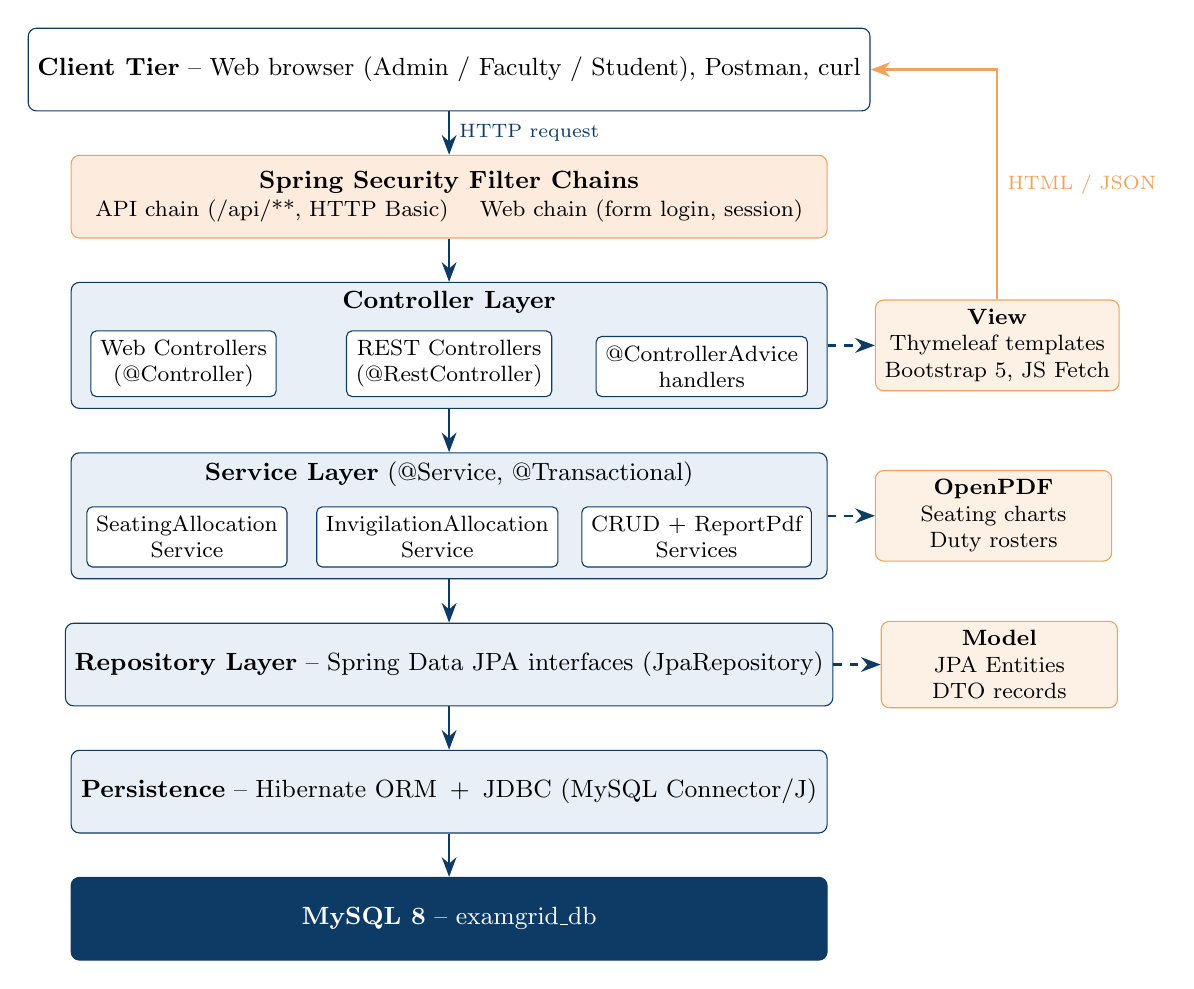
\begin{tikzpicture}[
  font=\small,
  layer/.style={draw=egnavy,fill=eglight,rounded corners=3pt,minimum width=9.6cm,minimum height=1.05cm,align=center},
  comp/.style={draw=egnavy,fill=white,rounded corners=2pt,minimum height=0.7cm,align=center,font=\footnotesize},
  side/.style={draw=eggold,fill=eggold!15,rounded corners=3pt,minimum width=3.0cm,minimum height=1.05cm,align=center,font=\footnotesize},
  arr/.style={-{Stealth[length=2.5mm]},thick,egnavy}]

\node[layer,fill=white] (client) {\textbf{Client Tier} -- Web browser (Admin / Faculty / Student), Postman, curl};
\node[layer,below=0.55cm of client,fill=eggold!20,draw=eggold] (sec) {\textbf{Spring Security Filter Chains}\\[-1pt]\footnotesize API chain (/api/**, HTTP Basic) \quad Web chain (form login, session)};
\node[layer,below=0.55cm of sec,minimum height=1.6cm] (ctl) {};
\node[anchor=north] at (ctl.north) {\textbf{Controller Layer}};
\node[comp,anchor=south west] at ([xshift=0.25cm,yshift=0.15cm]ctl.south west) {Web Controllers\\(@Controller)};
\node[comp,anchor=south] at ([yshift=0.15cm]ctl.south) {REST Controllers\\(@RestController)};
\node[comp,anchor=south east] at ([xshift=-0.25cm,yshift=0.15cm]ctl.south east) {@ControllerAdvice\\handlers};
\node[layer,below=0.55cm of ctl,minimum height=1.6cm] (svc) {};
\node[anchor=north] at (svc.north) {\textbf{Service Layer} (@Service, @Transactional)};
\node[comp,anchor=south west] at ([xshift=0.2cm,yshift=0.15cm]svc.south west) {SeatingAllocation\\Service};
\node[comp,anchor=south] at ([xshift=-0.15cm,yshift=0.15cm]svc.south) {InvigilationAllocation\\Service};
\node[comp,anchor=south east] at ([xshift=-0.2cm,yshift=0.15cm]svc.south east) {CRUD + ReportPdf\\Services};
\node[layer,below=0.55cm of svc] (repo) {\textbf{Repository Layer} -- Spring Data JPA interfaces (JpaRepository)};
\node[layer,below=0.55cm of repo] (orm) {\textbf{Persistence} -- Hibernate ORM \,+\, JDBC (MySQL Connector/J)};
\node[layer,below=0.55cm of orm,fill=egnavy,text=white] (db) {\textbf{MySQL 8} -- examgrid\_db};

\node[side,right=0.6cm of ctl] (view) {\textbf{View}\\Thymeleaf templates\\Bootstrap 5, JS Fetch};
\node[side,right=0.6cm of svc] (pdf) {\textbf{OpenPDF}\\Seating charts\\Duty rosters};
\node[side,right=0.6cm of repo] (ent) {\textbf{Model}\\JPA Entities\\DTO records};

\draw[arr] (client) -- node[right,font=\scriptsize]{HTTP request} (sec);
\draw[arr] (sec) -- (ctl);
\draw[arr] (ctl) -- (svc);
\draw[arr] (svc) -- (repo);
\draw[arr] (repo) -- (orm);
\draw[arr] (orm) -- (db);
\draw[arr,dashed] (ctl) -- (view);
\draw[arr,dashed] (svc) -- (pdf);
\draw[arr,dashed] (repo) -- (ent);
\draw[arr,eggold] (view.north) |- node[pos=0.25,right,font=\scriptsize]{HTML / JSON} (client.east);
\end{tikzpicture}
}
\caption{Layered architecture of ExamGrid}
\end{figure}

\subsection{Database Design}
The database \texttt{examgrid\_db} has seven tables. Foreign keys link every seat to a student, an exam and a hall, and every duty to a faculty member and a hall.
\begin{table}[H]
\begin{gridtable}{|L{3.2cm}|L{5.6cm}|X|}
\hline
\hd{Table} & \hd{Important columns} & \hd{Description}\\\hline
students & id, usn (unique), name, branch, semester, email & Students who write exams\\\hline
faculty & id, faculty\_code (unique), name, department, max\_duties & Invigilators and their duty limit\\\hline
halls & id, hall\_name (unique), block, total\_rows, total\_columns & Exam halls; capacity = rows $\times$ columns\\\hline
exams & id, subject\_code, subject\_name, branch, semester, exam\_date, start\_time, end\_time & Timetable; same date and start time form one slot\\\hline
seat\_allocations & id, exam\_id, student\_id, hall\_id, exam\_date, start\_time, seat\_row, seat\_column, seat\_number & One seat per student per exam\\\hline
invigilation\_duties & id, faculty\_id, hall\_id, exam\_date, start\_time, end\_time & Duty of a faculty member in a hall\\\hline
app\_users & id, username (unique), password, role, enabled & Login accounts; role is ADMIN, FACULTY or STUDENT\\\hline
\end{gridtable}
\caption{Database tables}
\end{table}
Two unique constraints on \texttt{seat\_allocations} guarantee that a student is seated only once per exam and that a physical seat is used only once per slot.
\begin{figure}[H]\centering
\resizebox{\linewidth}{!}{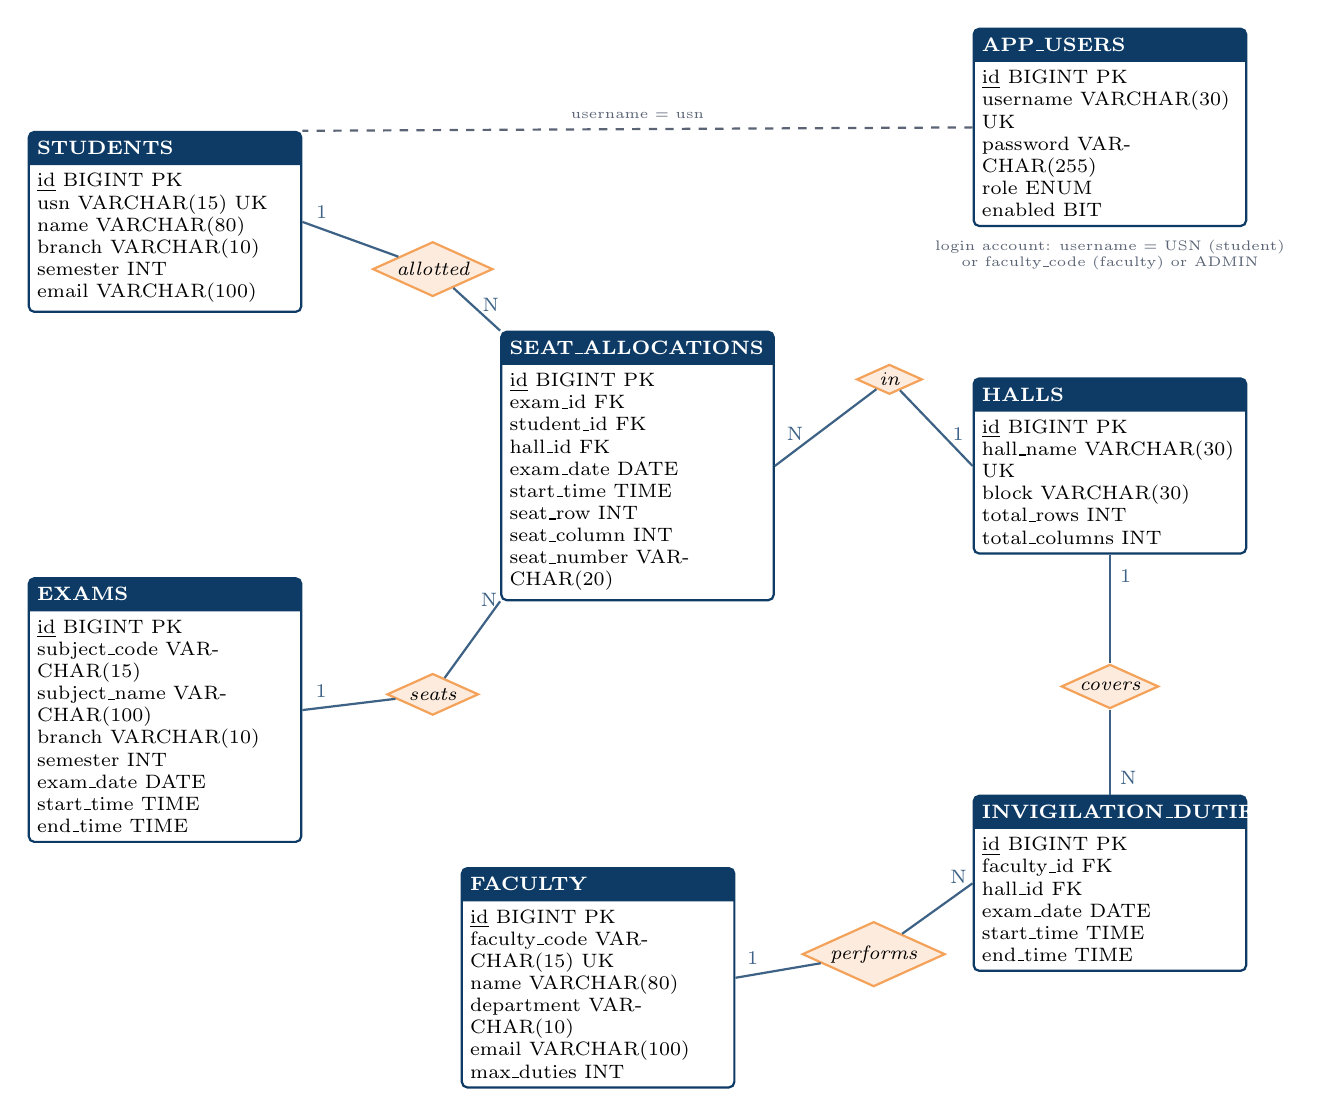
\begin{tikzpicture}[
  font=\scriptsize,
  ent/.style={rectangle split,rectangle split parts=2,draw=egnavy,thick,rounded corners=2pt,
              rectangle split part fill={egnavy,white},text width=3.25cm,align=left,inner sep=3pt},
  rel/.style={diamond,draw=eggold,fill=eggold!20,thick,aspect=2.2,inner sep=1pt,font=\scriptsize\itshape},
  ln/.style={thick,egnavy!80}]

\node[ent] (student) at (0,0) {\textcolor{white}{\textbf{STUDENTS}}\nodepart{two}
  \underline{id} BIGINT PK\\ usn VARCHAR(15) UK\\ name VARCHAR(80)\\ branch VARCHAR(10)\\ semester INT\\ email VARCHAR(100)};
\node[ent] (exam) at (0,-6.2) {\textcolor{white}{\textbf{EXAMS}}\nodepart{two}
  \underline{id} BIGINT PK\\ subject\_code VARCHAR(15)\\ subject\_name VARCHAR(100)\\ branch VARCHAR(10)\\ semester INT\\ exam\_date DATE\\ start\_time TIME\\ end\_time TIME};
\node[ent] (seat) at (6,-3.1) {\textcolor{white}{\textbf{SEAT\_ALLOCATIONS}}\nodepart{two}
  \underline{id} BIGINT PK\\ exam\_id FK\\ student\_id FK\\ hall\_id FK\\ exam\_date DATE\\ start\_time TIME\\ seat\_row INT\\ seat\_column INT\\ seat\_number VARCHAR(20)};
\node[ent] (hall) at (12,-3.1) {\textcolor{white}{\textbf{HALLS}}\nodepart{two}
  \underline{id} BIGINT PK\\ hall\_name VARCHAR(30) UK\\ block VARCHAR(30)\\ total\_rows INT\\ total\_columns INT};
\node[ent] (duty) at (12,-8.4) {\textcolor{white}{\textbf{INVIGILATION\_DUTIES}}\nodepart{two}
  \underline{id} BIGINT PK\\ faculty\_id FK\\ hall\_id FK\\ exam\_date DATE\\ start\_time TIME\\ end\_time TIME};
\node[ent] (faculty) at (5.5,-9.6) {\textcolor{white}{\textbf{FACULTY}}\nodepart{two}
  \underline{id} BIGINT PK\\ faculty\_code VARCHAR(15) UK\\ name VARCHAR(80)\\ department VARCHAR(10)\\ email VARCHAR(100)\\ max\_duties INT};
\node[ent] (user) at (12,1.2) {\textcolor{white}{\textbf{APP\_USERS}}\nodepart{two}
  \underline{id} BIGINT PK\\ username VARCHAR(30) UK\\ password VARCHAR(255)\\ role ENUM\\ enabled BIT};

\node[rel] (r1) at (3.4,-0.6) {allotted};
\node[rel] (r2) at (3.4,-6.0) {seats};
\node[rel] (r3) at (9.2,-2.0) {in};
\node[rel] (r4) at (12,-5.9) {covers};
\node[rel] (r5) at (9.0,-9.3) {performs};

\draw[ln] (student.east) -- node[above,pos=0.2]{1} (r1) -- node[above,pos=0.8]{N} (seat.north west);
\draw[ln] (exam.east) -- node[above,pos=0.2]{1} (r2) -- node[above,pos=0.8]{N} (seat.south west);
\draw[ln] (hall.west) -- node[above,pos=0.2]{1} (r3) -- node[above,pos=0.8]{N} (seat.east);
\draw[ln] (hall.south) -- node[right,pos=0.2]{1} (r4) -- node[right,pos=0.8]{N} (duty.north);
\draw[ln] (faculty.east) -- node[above,pos=0.2]{1} (r5) -- node[above,pos=0.8]{N} (duty.west);
\draw[ln,dashed,eggrey] (user.west) -- node[above,font=\tiny,align=center]{username = usn}  (student.north east);
\node[font=\tiny,eggrey,align=center,below=1pt of user] {login account: username = USN (student)\\or faculty\_code (faculty) or ADMIN};
\end{tikzpicture}
}
\caption{Entity-relationship diagram}
\end{figure}

\subsection{Authentication and Authorisation}
When the exam cell adds a student or faculty member, a login account is created automatically with the USN or faculty code as the username and a default password. Passwords are never stored in plain text: Spring Security's \texttt{BCryptPasswordEncoder} stores a salted hash. \texttt{AppUserDetailsService} loads the account at login, and after a successful login the user is redirected to a page for their role.

Two security filter chains are configured. The chain for \texttt{/api/**} uses HTTP Basic authentication so that Postman and curl can call the API; seat lookup is public, a faculty member may read only his or her own roster, and all other API calls need the exam cell role. The chain for the web pages uses a custom login page, CSRF protection, session fixation protection and one active session per user. Opening a page meant for another role shows an access-denied page.

\subsection{Seating Allocation Algorithm}
All exams with the same date and start time form a \emph{slot}. For a slot, \texttt{SeatingAllocationService} builds one queue of students per exam (all students of the exam's branch and semester) and checks that the total number of students does not exceed the total hall capacity; otherwise it stops with an \texttt{InsufficientCapacityException}. It then fills the halls, largest first, seat by seat and row by row. For each seat it looks at the already-filled left and front neighbours and chooses the exam with the most waiting students whose subject and branch differ from both. If none exists it relaxes the branch rule; if still none exists it leaves the seat empty while spare seats remain, and only places the student next to the same subject when there is no other way to seat everyone, counting it as a clash.
\begin{figure}[H]\centering
\resizebox{!}{0.55\textheight}{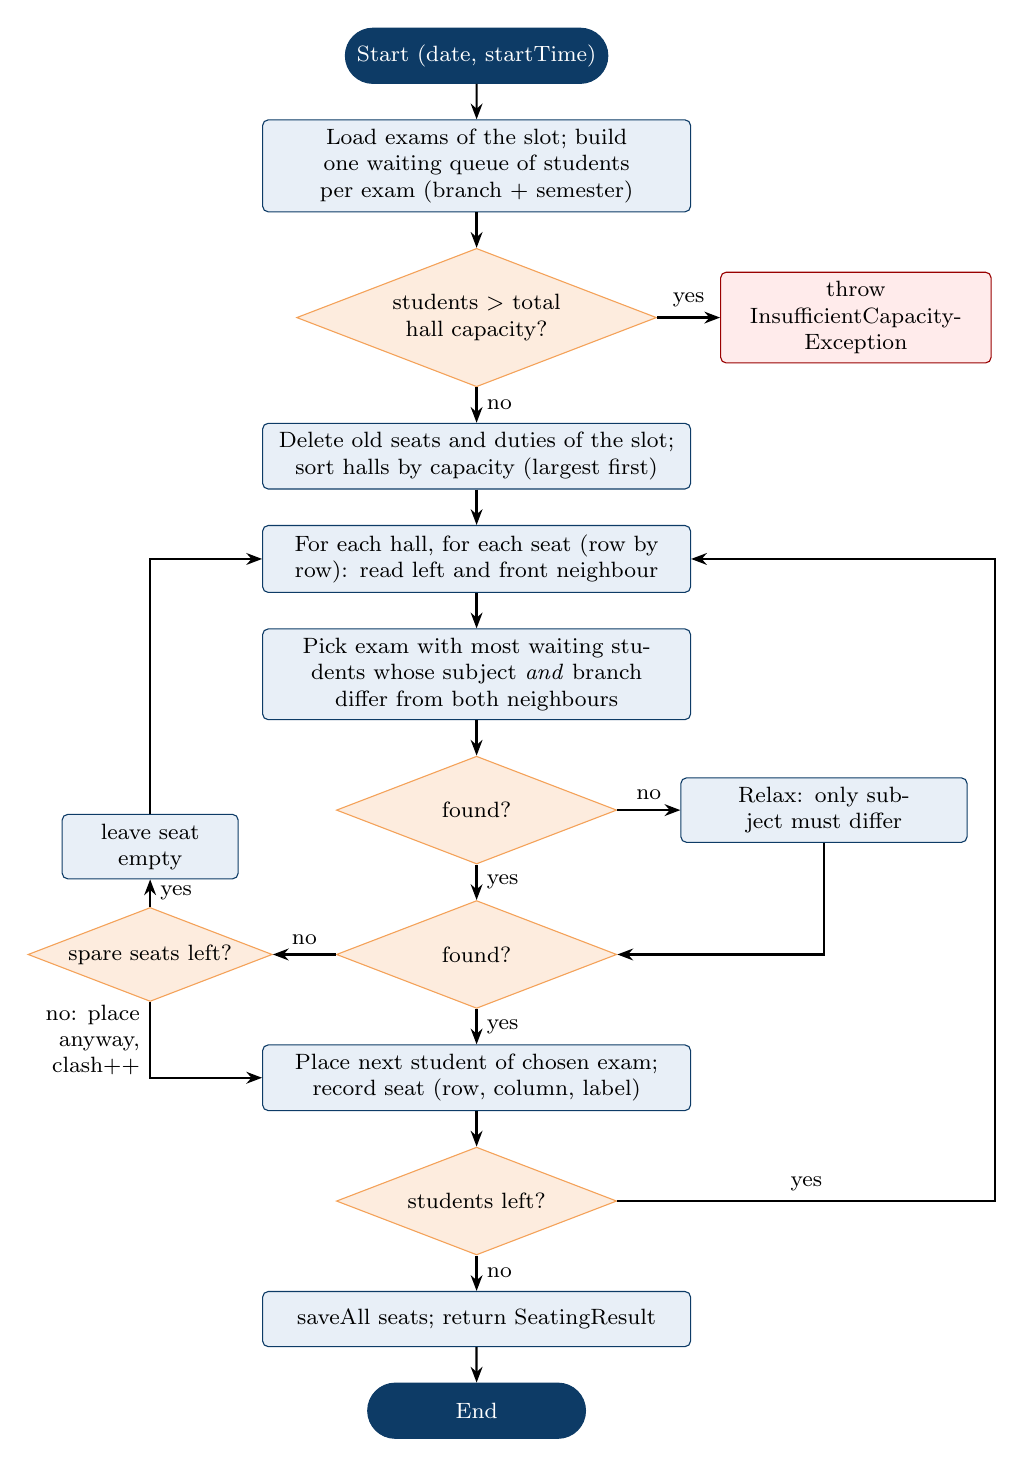
\begin{tikzpicture}[
  font=\footnotesize, node distance=0.45cm,
  term/.style={rounded rectangle,draw=egnavy,fill=egnavy,text=white,minimum height=0.7cm,minimum width=3cm},
  proc/.style={rectangle,draw=egnavy,fill=eglight,rounded corners=2pt,minimum height=0.7cm,text width=5.2cm,align=center},
  dec/.style={diamond,draw=eggold,fill=eggold!20,aspect=2.6,inner sep=1pt,text width=2.8cm,align=center},
  err/.style={rectangle,draw=red!60!black,fill=red!8,rounded corners=2pt,text width=3.2cm,align=center,minimum height=0.7cm},
  arr/.style={-{Stealth[length=2mm]},thick}]
\node[term] (s) {Start (date, startTime)};
\node[proc,below=of s] (p1) {Load exams of the slot; build one waiting queue of students per exam (branch + semester)};
\node[dec,below=of p1] (d1) {students $>$ total hall capacity?};
\node[err,right=0.8cm of d1] (e1) {throw InsufficientCapacity\-Exception};
\node[proc,below=of d1] (p2) {Delete old seats and duties of the slot; sort halls by capacity (largest first)};
\node[proc,below=of p2] (p3) {For each hall, for each seat (row by row): read left and front neighbour};
\node[proc,below=of p3] (p4) {Pick exam with most waiting students whose subject \emph{and} branch differ from both neighbours};
\node[dec,below=of p4] (d2) {found?};
\node[proc,right=0.8cm of d2,text width=3.4cm] (p5) {Relax: only subject must differ};
\node[dec,below=of d2] (d3) {found?};
\node[dec,left=0.8cm of d3,text width=2.2cm] (d4) {spare seats left?};
\node[proc,above=0.35cm of d4,text width=2.0cm] (skip) {leave seat empty};
\node[proc,below=of d3] (p6) {Place next student of chosen exam; record seat (row, column, label)};
\node[dec,below=of p6] (d5) {students left?};
\node[proc,below=of d5] (p7) {saveAll seats; return SeatingResult};
\node[term,below=of p7] (e) {End};

\draw[arr] (s)--(p1); \draw[arr] (p1)--(d1);
\draw[arr] (d1)--node[above]{yes}(e1);
\draw[arr] (d1)--node[right]{no}(p2);
\draw[arr] (p2)--(p3); \draw[arr] (p3)--(p4); \draw[arr] (p4)--(d2);
\draw[arr] (d2)--node[right]{yes}(d3);
\draw[arr] (d2)--node[above]{no}(p5);
\draw[arr] (p5) |- (d3);
\draw[arr] (d3)--node[right]{yes}(p6);
\draw[arr] (d3)--node[above]{no}(d4);
\draw[arr] (d4)--node[right]{yes}(skip);
\draw[arr] (d4) |- node[pos=0.25,left,align=right]{no: place\\anyway,\\clash++} (p6.west);
\draw[arr] (skip.north) |- (p3.west);
\draw[arr] (p6)--(d5);
\draw[arr] (d5)--node[right]{no}(p7);
\draw[arr] (d5.east) -- node[above]{yes} ++(4.8,0) |- (p3.east);
\draw[arr] (p7)--(e);
\end{tikzpicture}
}
\caption{Seating allocation flowchart}
\end{figure}
Because each seat is compared with its left and front neighbours at the time it is filled, no two adjacent seats ever hold the same subject when space allows. Choosing the largest waiting group first keeps the queues balanced, so the last seats are not left with a single subject.
\begin{figure}[H]\centering
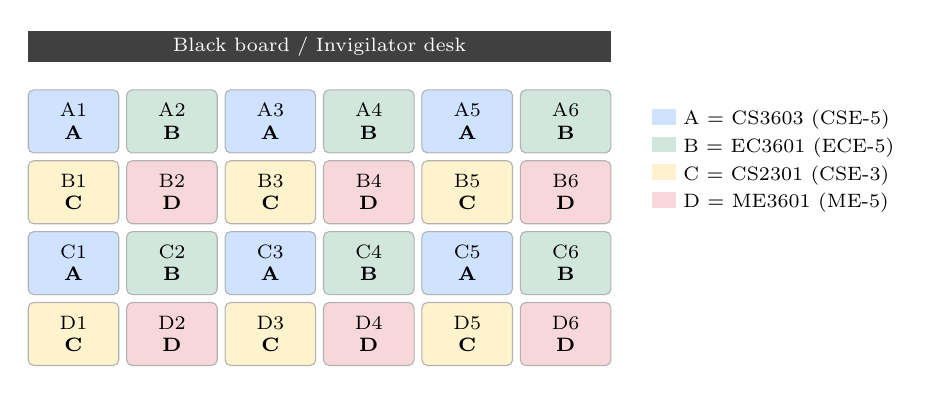
\begin{tikzpicture}[font=\scriptsize]
\definecolor{sA}{RGB}{207,226,255}
\definecolor{sB}{RGB}{209,231,221}
\definecolor{sC}{RGB}{255,243,205}
\definecolor{sD}{RGB}{248,215,218}
\fill[black!75] (0,0.35) rectangle (6*1.25-0.1,0.75);
\node[white] at (3.7,0.55) {Black board / Invigilator desk};
\foreach \s [count=\i from 0] in {A,B,A,B,A,B,C,D,C,D,C,D,A,B,A,B,A,B,C,D,C,D,C,D}{
  \pgfmathtruncatemacro{\r}{int(\i/6)}
  \pgfmathtruncatemacro{\c}{mod(\i,6)}
  \pgfmathtruncatemacro{\cc}{\c+1}
  \fill[s\s,draw=black!30,rounded corners=2pt] (\c*1.25,-\r*0.9) rectangle ++(1.15,-0.8);
  \node[align=center] at (\c*1.25+0.575,-\r*0.9-0.4) {\ifcase\r A\or B\or C\or D\fi\cc\\\textbf{\s}};
}
\node[anchor=west,align=left] at (7.8,-0.9) {
  \tikz\fill[sA](0,0)rectangle(0.3,0.2); A = CS3603 (CSE-5)\\[2pt]
  \tikz\fill[sB](0,0)rectangle(0.3,0.2); B = EC3601 (ECE-5)\\[2pt]
  \tikz\fill[sC](0,0)rectangle(0.3,0.2); C = CS2301 (CSE-3)\\[2pt]
  \tikz\fill[sD](0,0)rectangle(0.3,0.2); D = ME3601 (ME-5)};
\end{tikzpicture}

\caption{Illustrative seating pattern; equal letters never touch}
\end{figure}

\subsection{Invigilation Allocation Algorithm}
After seating, \texttt{InvigilationAllocationService} counts the students in each used hall and requires one invigilator for every 30 students (at least one). For each required invigilator it considers only faculty who have not reached their maximum duties and who have no duty overlapping the slot on that date, and picks the one with the fewest duties so far. Two duties overlap when one starts before the other ends. If no faculty member is free, an \texttt{AllocationException} is thrown and the transaction rolls back, so no partial roster is saved.
\begin{figure}[H]\centering
\resizebox{!}{0.5\textheight}{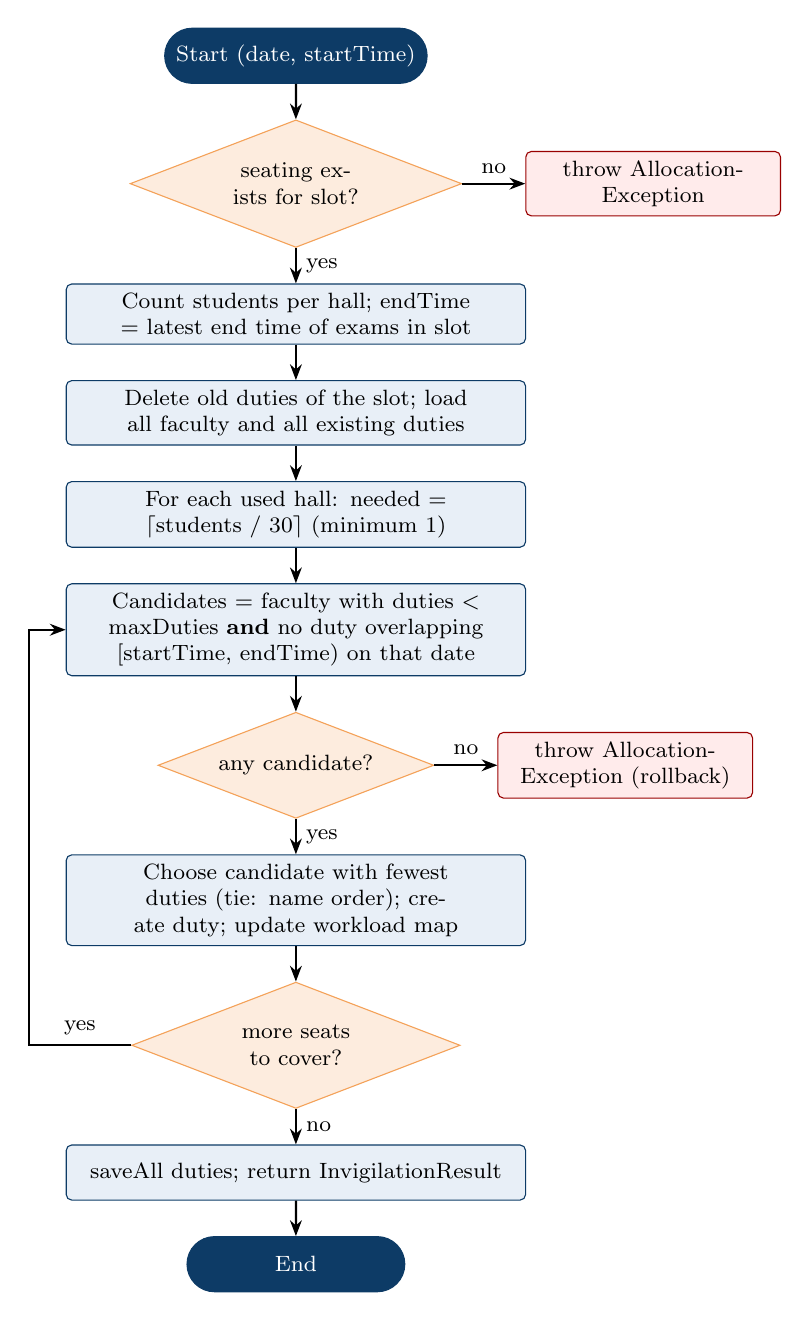
\begin{tikzpicture}[
  font=\footnotesize, node distance=0.45cm,
  term/.style={rounded rectangle,draw=egnavy,fill=egnavy,text=white,minimum height=0.7cm,minimum width=3cm},
  proc/.style={rectangle,draw=egnavy,fill=eglight,rounded corners=2pt,minimum height=0.7cm,text width=5.6cm,align=center},
  dec/.style={diamond,draw=eggold,fill=eggold!20,aspect=2.6,inner sep=1pt,text width=2.6cm,align=center},
  err/.style={rectangle,draw=red!60!black,fill=red!8,rounded corners=2pt,text width=3.0cm,align=center,minimum height=0.7cm},
  arr/.style={-{Stealth[length=2mm]},thick}]
\node[term] (s) {Start (date, startTime)};
\node[dec,below=of s] (d0) {seating exists for slot?};
\node[err,right=0.8cm of d0] (e0) {throw Allocation\-Exception};
\node[proc,below=of d0] (p1) {Count students per hall; endTime = latest end time of exams in slot};
\node[proc,below=of p1] (p2) {Delete old duties of the slot; load all faculty and all existing duties};
\node[proc,below=of p2] (p3) {For each used hall: needed = $\lceil$students / 30$\rceil$ (minimum 1)};
\node[proc,below=of p3] (p4) {Candidates = faculty with duties $<$ maxDuties \textbf{and} no duty overlapping [startTime, endTime) on that date};
\node[dec,below=of p4] (d1) {any candidate?};
\node[err,right=0.8cm of d1] (e1) {throw Allocation\-Exception (rollback)};
\node[proc,below=of d1] (p5) {Choose candidate with fewest duties (tie: name order); create duty; update workload map};
\node[dec,below=of p5] (d2) {more seats to cover?};
\node[proc,below=of d2] (p6) {saveAll duties; return InvigilationResult};
\node[term,below=of p6] (e) {End};
\draw[arr] (s)--(d0);
\draw[arr] (d0)--node[above]{no}(e0);
\draw[arr] (d0)--node[right]{yes}(p1);
\draw[arr] (p1)--(p2); \draw[arr] (p2)--(p3); \draw[arr] (p3)--(p4); \draw[arr] (p4)--(d1);
\draw[arr] (d1)--node[above]{no}(e1);
\draw[arr] (d1)--node[right]{yes}(p5);
\draw[arr] (p5)--(d2);
\draw[arr] (d2)--node[right]{no}(p6);
\draw[arr] (d2.west) -- node[above]{yes} ++(-1.3,0) |- (p4.west);
\draw[arr] (p6)--(e);
\end{tikzpicture}
}
\caption{Invigilation allocation flowchart}
\end{figure}

\subsection{Modules}
\textbf{Exam cell module.} The dashboard shows counts of students, faculty, halls, seats and exams, the upcoming exam slots and the workload of each faculty member. Separate pages manage students, faculty, halls and exams; each has a form with field-level validation messages and a searchable table with edit and delete actions. The allocation page lists every slot with buttons to generate seating, assign invigilators, view the plan and download the seating PDF. The seating plan page shows each hall as a colour-coded grid, and the duties page shows the roster with a date filter and a PDF download.

\textbf{Faculty module.} After login a faculty member sees his or her own invigilation duties with date, time, hall and block. The page loads the roster from \texttt{/api/duties/faculty/\{code\}} using the Fetch API.

\textbf{Student module.} A student can enter a USN on the public seat lookup page, or log in to see his or her seats automatically. Each result card shows the subject, date, time, hall, block, row, bench and seat number.

\textbf{Reports.} \texttt{ReportPdfService} builds a seating chart PDF with one grid page and one attendance sheet per hall, and a duty roster PDF with a signature column.

\subsection{Validation and Exception Handling}
Entities carry Bean Validation annotations such as \texttt{@NotBlank}, \texttt{@Pattern} for the USN, \texttt{@Min}/\texttt{@Max} for semester and hall size, and \texttt{@Email}. Controllers check them with \texttt{@Valid}. The exam service also rejects an exam whose end time is not after its start time, or which overlaps another exam of the same branch and semester. Custom exceptions (\texttt{ResourceNotFoundException}, \texttt{DuplicateResourceException}, \texttt{InsufficientCapacityException}, \texttt{AllocationException}, \texttt{InvalidRequestException}) are handled in one place: \texttt{ApiExceptionHandler} returns a JSON error body with the correct HTTP status, and \texttt{WebExceptionHandler} shows an error page.

\subsection{REST API}
\begin{table}[H]
\begin{gridtable}{|L{2.7cm}|X|L{3.2cm}|}
\hline
\hd{Method} & \hd{Endpoint} & \hd{Access}\\\hline
GET, POST & /api/students, /api/faculty, /api/halls, /api/exams & Exam cell\\\hline
GET, PUT, DELETE & /api/\{resource\}/\{id\} & Exam cell\\\hline
POST, GET & /api/allocations/seating?date=\&startTime= & Exam cell\\\hline
POST & /api/allocations/invigilation?date=\&startTime= & Exam cell\\\hline
GET & /api/seats/\{usn\} & Public\\\hline
GET & /api/duties/faculty/\{code\} & Exam cell, own faculty\\\hline
GET & /api/duties, /api/duties/workload & Exam cell\\\hline
\end{gridtable}
\caption{Main REST endpoints}
\end{table}
Example request with curl:
\begin{lstlisting}[style=plain]
curl -u admin:admin123 -X POST "http://localhost:8080/api/allocations/seating?date=2026-12-07&startTime=09:30"
curl http://localhost:8080/api/seats/NNM24CS224
\end{lstlisting}

\subsection{Testing}
JUnit 5 tests run on the full Spring context with an in-memory H2 database and the sample data. \texttt{SeatingAllocationServiceTest} checks that every student gets exactly one seat, that no hall exceeds its capacity, that no neighbours write the same subject, and that too-small halls are rejected. \texttt{InvigilationAllocationServiceTest} checks clash-free duties, the 30-students rule, the duty limit and workload balance. \texttt{ApiControllerTest} uses MockMvc to check the public lookup, the 401/403 responses, validation errors and that a faculty member cannot read another faculty member's roster. The tests are run with \texttt{mvn test}; the APIs were also tested manually with Postman and curl.

\chapter{Results and Discussion}
ExamGrid was built with Maven, run with \texttt{mvn spring-boot:run} and tested with the sample data that the application loads into MySQL on first start: 148 students of four classes, four halls with 192 seats, ten faculty members and eight exams in three slots. The application is opened at \texttt{http://localhost:8080}. The following screens show the main features.

\screenshot{01_home}{Home page}
\screenshot{02_login}{Login page}
\screenshot{03_admin_dashboard}{Exam cell dashboard}
\screenshot{04_students}{Student management with validation}
\screenshot{05_halls}{Hall management}
\screenshot{06_exams}{Exam timetable}
\screenshot{07_allocation}{Allocation page with exam slots}
\screenshot{08_seating_plan}{Generated seating plan, one colour per subject}
\screenshot{09_duties}{Invigilation duty roster and workload balance}
\screenshot{10_seating_pdf}{Seating chart PDF}
\screenshot{11_seat_lookup}{Public seat lookup by USN}
\screenshot{12_faculty_duties}{Faculty view of own duties}
\screenshot{13_postman}{Seat lookup API tested in Postman}

\subsection*{Discussion}
The allocation rules give the following results on the sample data:
\begin{table}[H]
\begin{gridtable}{|L{3.6cm}|L{1.4cm}|L{1.8cm}|X|L{2.2cm}|}
\hline
\hd{Slot} & \hd{Exams} & \hd{Students} & \hd{Halls used} & \hd{Same-subject neighbours}\\\hline
07-12-2026, 09:30 & 4 & 148 & SH-01 (64), LH-201 (56), LH-101 (28) & 0\\\hline
08-12-2026, 09:30 & 3 & 108 & SH-01 (64), LH-201 (44) & 0\\\hline
08-12-2026, 14:00 & 1 & 40 & SH-01 (32), LH-201 (8) & 0\\\hline
\end{gridtable}
\caption{Seating results on the sample data}
\end{table}
Every student was seated exactly once and no hall was over-filled. When several subjects shared a slot, students of the same subject were never placed next to each other; for the single-subject slot the engine left alternate seats empty, producing a chessboard pattern. If the halls were too small, the exam cell got a clear message and the old plan stayed unchanged.

For invigilation, the three slots needed 14 duties. No faculty member received two duties in the same slot, and the workload difference between the busiest and the least busy faculty member was one duty. A faculty member who opened another faculty member's roster through the API got a 403 response, and a student who opened an exam cell page was shown the access-denied page. Because all data lives in one database, the seating chart, the duty roster, the student lookup and the faculty view always show the same allocation, which was not possible with separate spreadsheets.

\chapter{Conclusion and Future Scope}
\subsection*{Conclusion}
ExamGrid automates exam seating and invigilation allocation at Nitte. The exam cell generates a conflict-free seating plan and a balanced, clash-free duty roster for each exam slot in seconds instead of hours, students find their seat by USN and faculty see their duties online. The project applied the main concepts of the Spring Framework: Spring Boot for configuration, Spring MVC and Thymeleaf for the user interface, Spring Data JPA and Hibernate with MySQL for persistence, Spring Security for role-based access, Bean Validation and \texttt{@ControllerAdvice} for robust input and error handling, and a layered architecture that keeps the allocation rules in two clean service classes.

\subsection*{Future Scope}
\begin{itemize}
  \item E-mail and SMS notification of seats and duties to students and faculty.
  \item Bulk import of students and the exam timetable from CSV or Excel files.
  \item Support for students with special needs, such as ground-floor halls and reserved seats.
  \item A rule to avoid assigning faculty to invigilate exams of their own subject.
  \item QR codes on admit cards that open the student's seat details.
  \item Attendance marking in the hall through a mobile view for invigilators.
  \item Deployment on the college server with HTTPS and scheduled database backups.
\end{itemize}

\chapter{References}
\begin{enumerate}[label={[\arabic*]},leftmargin=1cm,itemsep=6pt]
  \item Craig Walls, \emph{Spring in Action}, 6th Edition, Manning Publications, 2022.
  \item Herbert Schildt, \emph{Java: The Complete Reference}, 12th Edition, McGraw Hill Education, 2021.
  \item Spring Boot Reference Documentation, \url{https://docs.spring.io/spring-boot/}
  \item Spring Security Reference Documentation, \url{https://docs.spring.io/spring-security/reference/}
  \item Spring Data JPA Reference Documentation, \url{https://docs.spring.io/spring-data/jpa/reference/}
  \item Thymeleaf Documentation, \url{https://www.thymeleaf.org/documentation.html}
  \item MySQL 8.0 Reference Manual, Oracle Corporation, \url{https://dev.mysql.com/doc/refman/8.0/en/}
  \item OpenPDF Library, \url{https://github.com/LibrePDF/OpenPDF}
\end{enumerate}

\end{document}
